\documentclass[../main.tex]{subfiles}
 
\begin{document}

% overview of the methodology

This section discusses the data generation process and the resulting features and observations. Additionally, it details the machine learning process. Specifically, it explains the model fitting procedure, to include partitioning, validation, and other \ac{ml} design choices. The section also describes the evaluation procedure: how we compare different models, how we compute results, and how we analyze the results.

\subsection{Data}

% describe where the data came from

The data are generated by the \ac{avas}, an \ac{afrl}-developed military flight simulator that employs real-world physics and flight dynamics for \ac{usaf} research purposes. To create the dataset, the simulator is repeatedly guided through takeoff and various midair maneuvers. The simulator generates about $500$ observations per minute, so, by documenting the relative start and end times of a maneuver, the datapoints can be easily segregated and labeled. By turning for $n$ seconds, taking off for $n$ seconds, and flying (approximately) straight and level for $n$ seconds, we can balance the distribution of the three classes and generate a sizable dataset. The \ac{avas} source code was modified for this research so that it outputs the observations directly to a properly-formatted comma-separated values file; thus, the generated file is ready for \ac{ml}.

% how many observations/features per observation in a dataframe?
% describe the nature of the features

Fortunately, the availability of the \ac{avas} allows us to generate arbitrary amounts of data. For this research, $5,000$ observations constitute a sufficiently-large dataset. Each observation includes nine different flying metrics and a timestamp relative to the start of the simulation. The metrics are roll, pitch, and yaw (each in radians), altitude (in feet), airspeed and vertical velocity (in feet per second), and acceleration in each of three axes (in feet per second per second). The roll and pitch values range from $-\pi$ to $\pi$; yaw ranges from $0$ to $2\pi$; the altitude and airspeed are both greater than zero; the vertical velocity and accelerations are real number values. The timestamp data is only useful for labeling, so it is removed prior to fitting the models.

% what info is contained in the supervised learning label?

When flying the simulator, the maneuver performed during a given time period is noted, and all observations within this window are labeled with the maneuver in question; in doing so, the truth data is identified. Thus, the truth data are labeled according to the beliefs of the individual operating the simulator. Because this individual is not well-versed in aircraft flight, it is assumed that these labels are not always correct.

% how many classes? what is the distribution of observations?

The dataset has three classes: \textit{taking off}, \textit{turning}, and \textit{cruising}. By repeating the simulations with different starting conditions, we are able to balance the presence of each of the three classes in the dataset. Because the dataset is so large, we are also able to selectively filter the data to achieve different class distributions (if desired).

% data exploration (correlations, pair plots, histograms)

\figurename \ \ref{fig:hist} shows nine different histograms, one for each feature. These histograms illustrate the distribution of the features over all observations. Roll, pitch, vertical velocity, y-axis acceleration, and z-axis acceleration are all relatively uniformly-distributed (perhaps with some skewing). The remaining features are not uniformly-distributed.

Clearly, the values of the features cover significantly different ranges. For this reason, all features are scaled to ensure each feature is important in our model formulation. Scaling is completed in the data pre-processing phase.

\begin{figure}
    \centerline{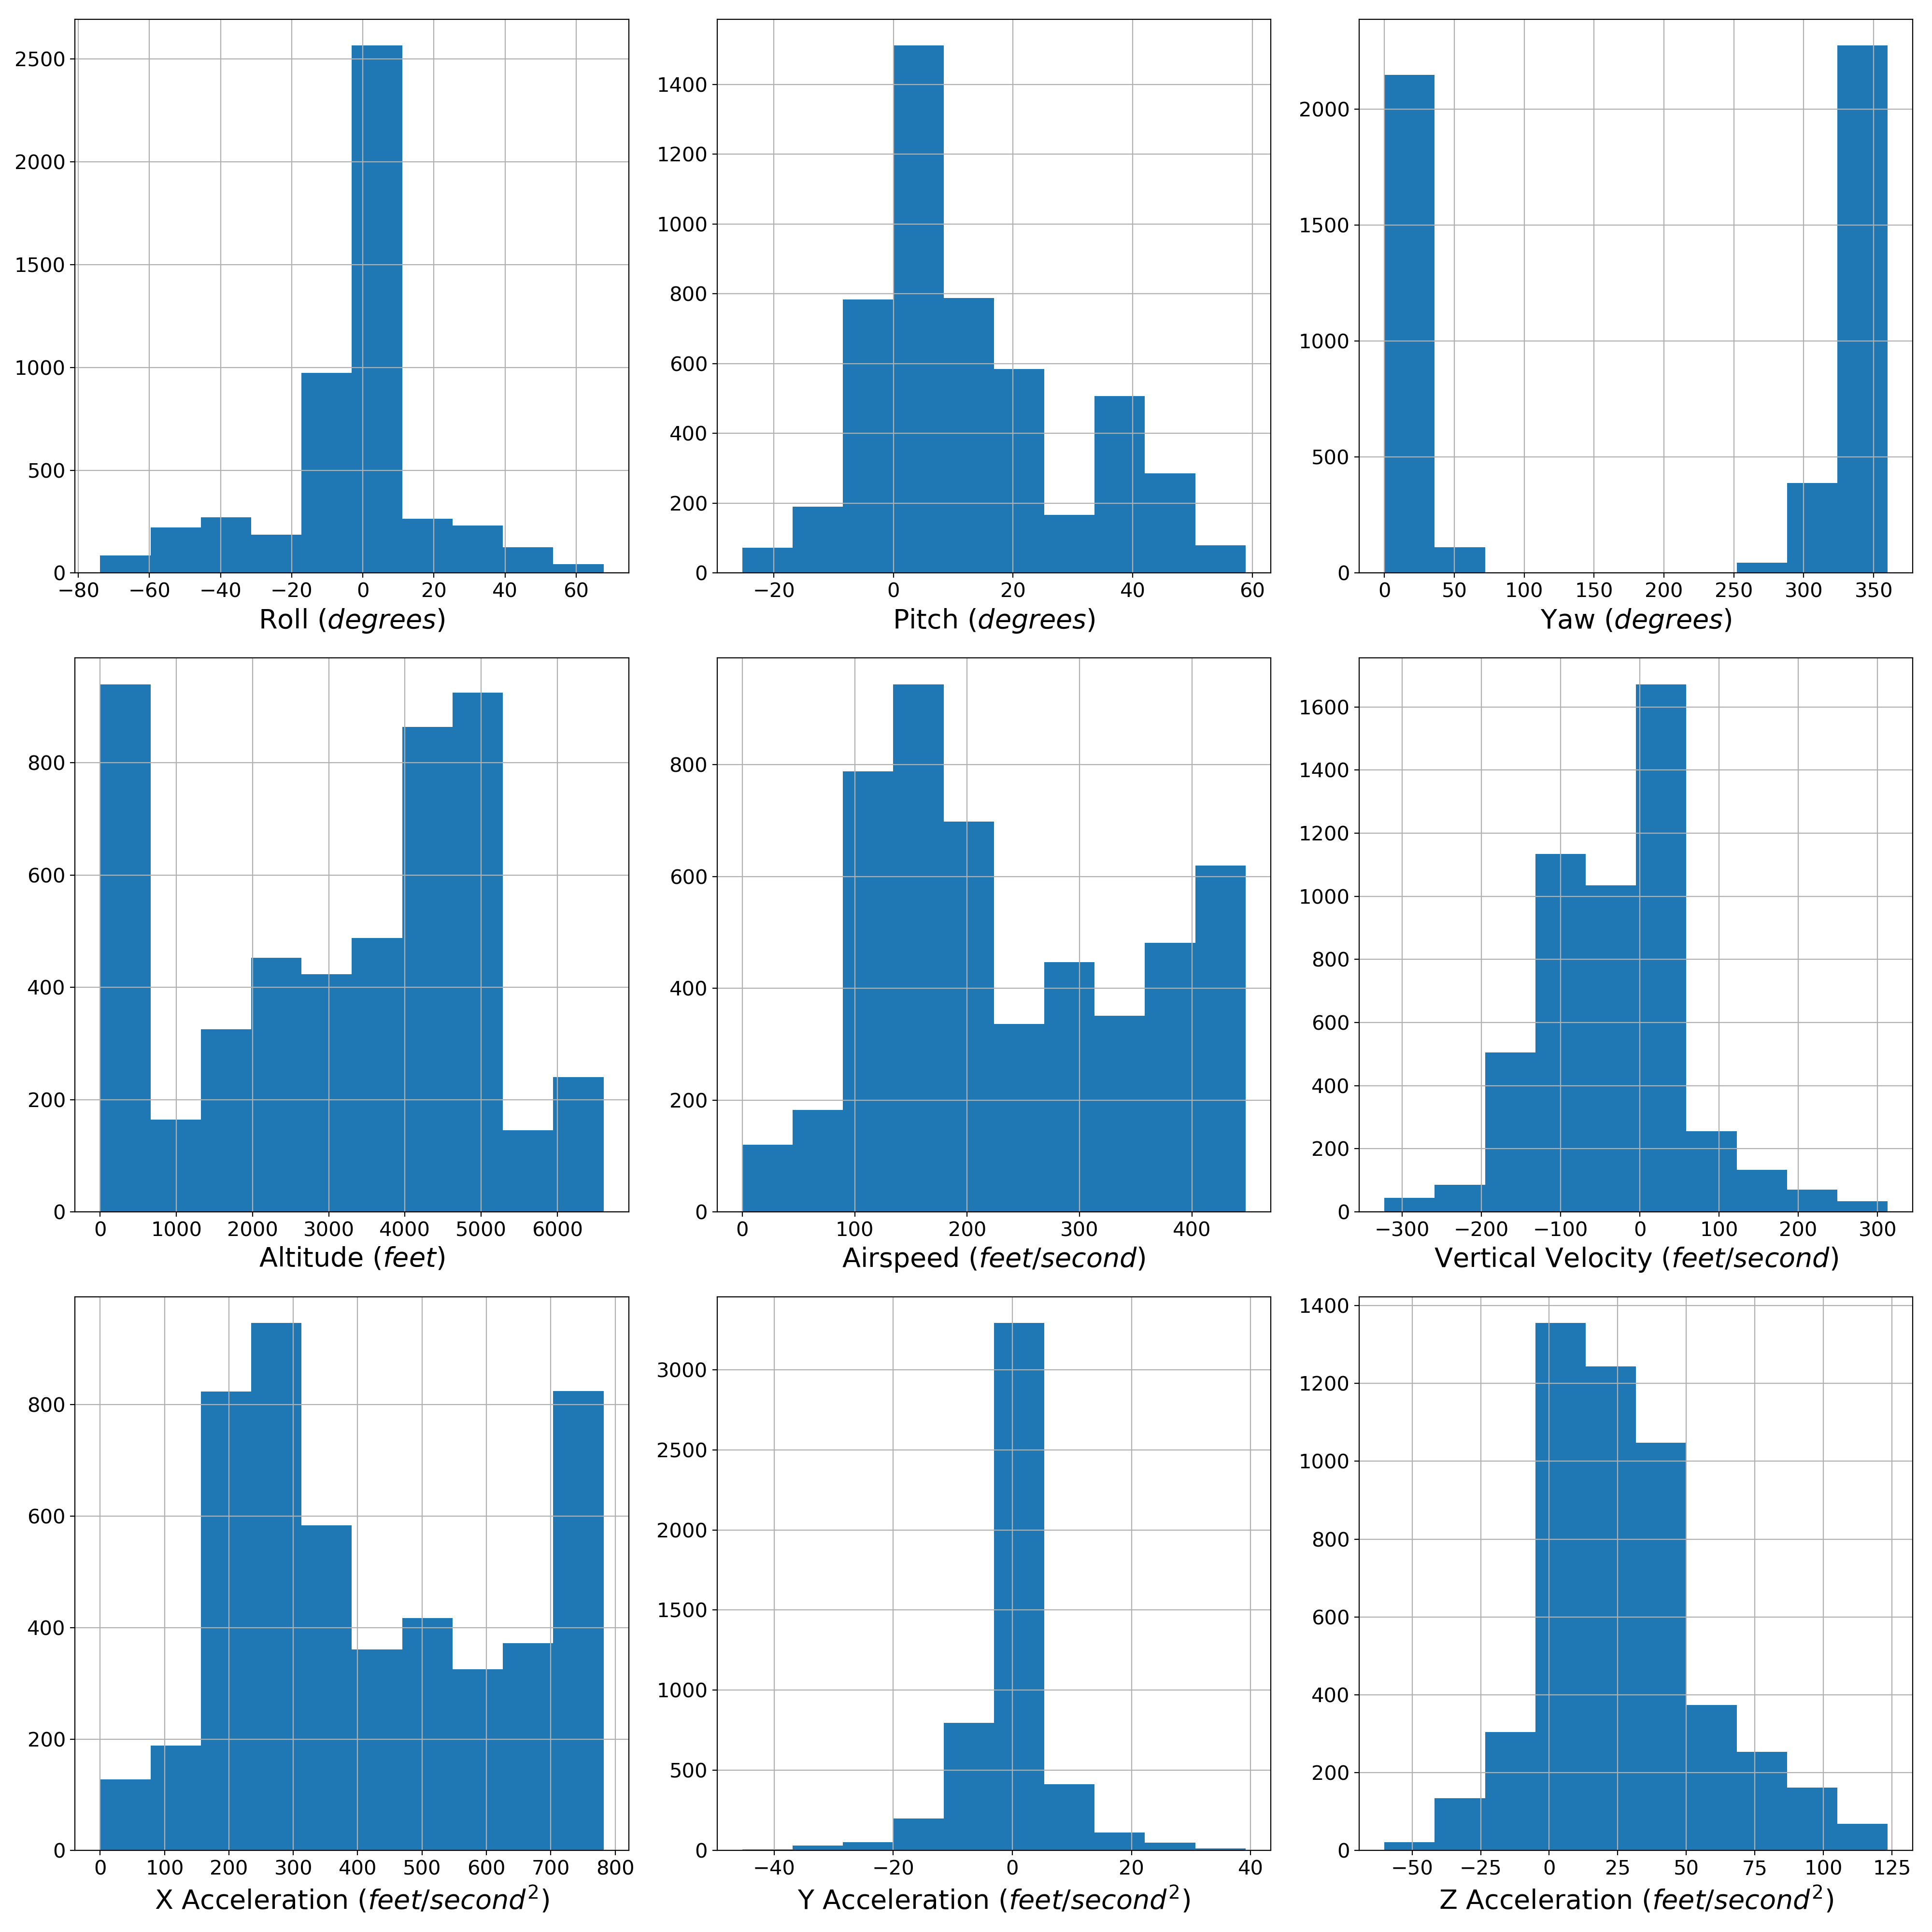
\includegraphics[width=\columnwidth]{all-feature-histogram.png}}
    \caption{A histogram for each feature. From left to right, top to bottom: roll, pitch, yaw, altitude, airspeed, vertical velocity, x-axis acceleration, y-axis acceleration, z-axis acceleration. The roll, pitch, and yaw values are shown in degrees to allow for greater interpretability.}
    \label{fig:hist}
\end{figure}

In \figurename \ \ref{fig:3d-plots}, each of three disparate groups of features are plotted on a \ac{3d} plot. Each group contains related features; for example, the first group contains roll, pitch, and yaw. As we examine the plots from left to right, it is clear that the boundaries between the classes grow less distinct. Thus, we predict that the features in the left plot outperform those in the middle plot, and we expect those in the middle plot to outperform those in the right plot.

\begin{figure}
    \centerline{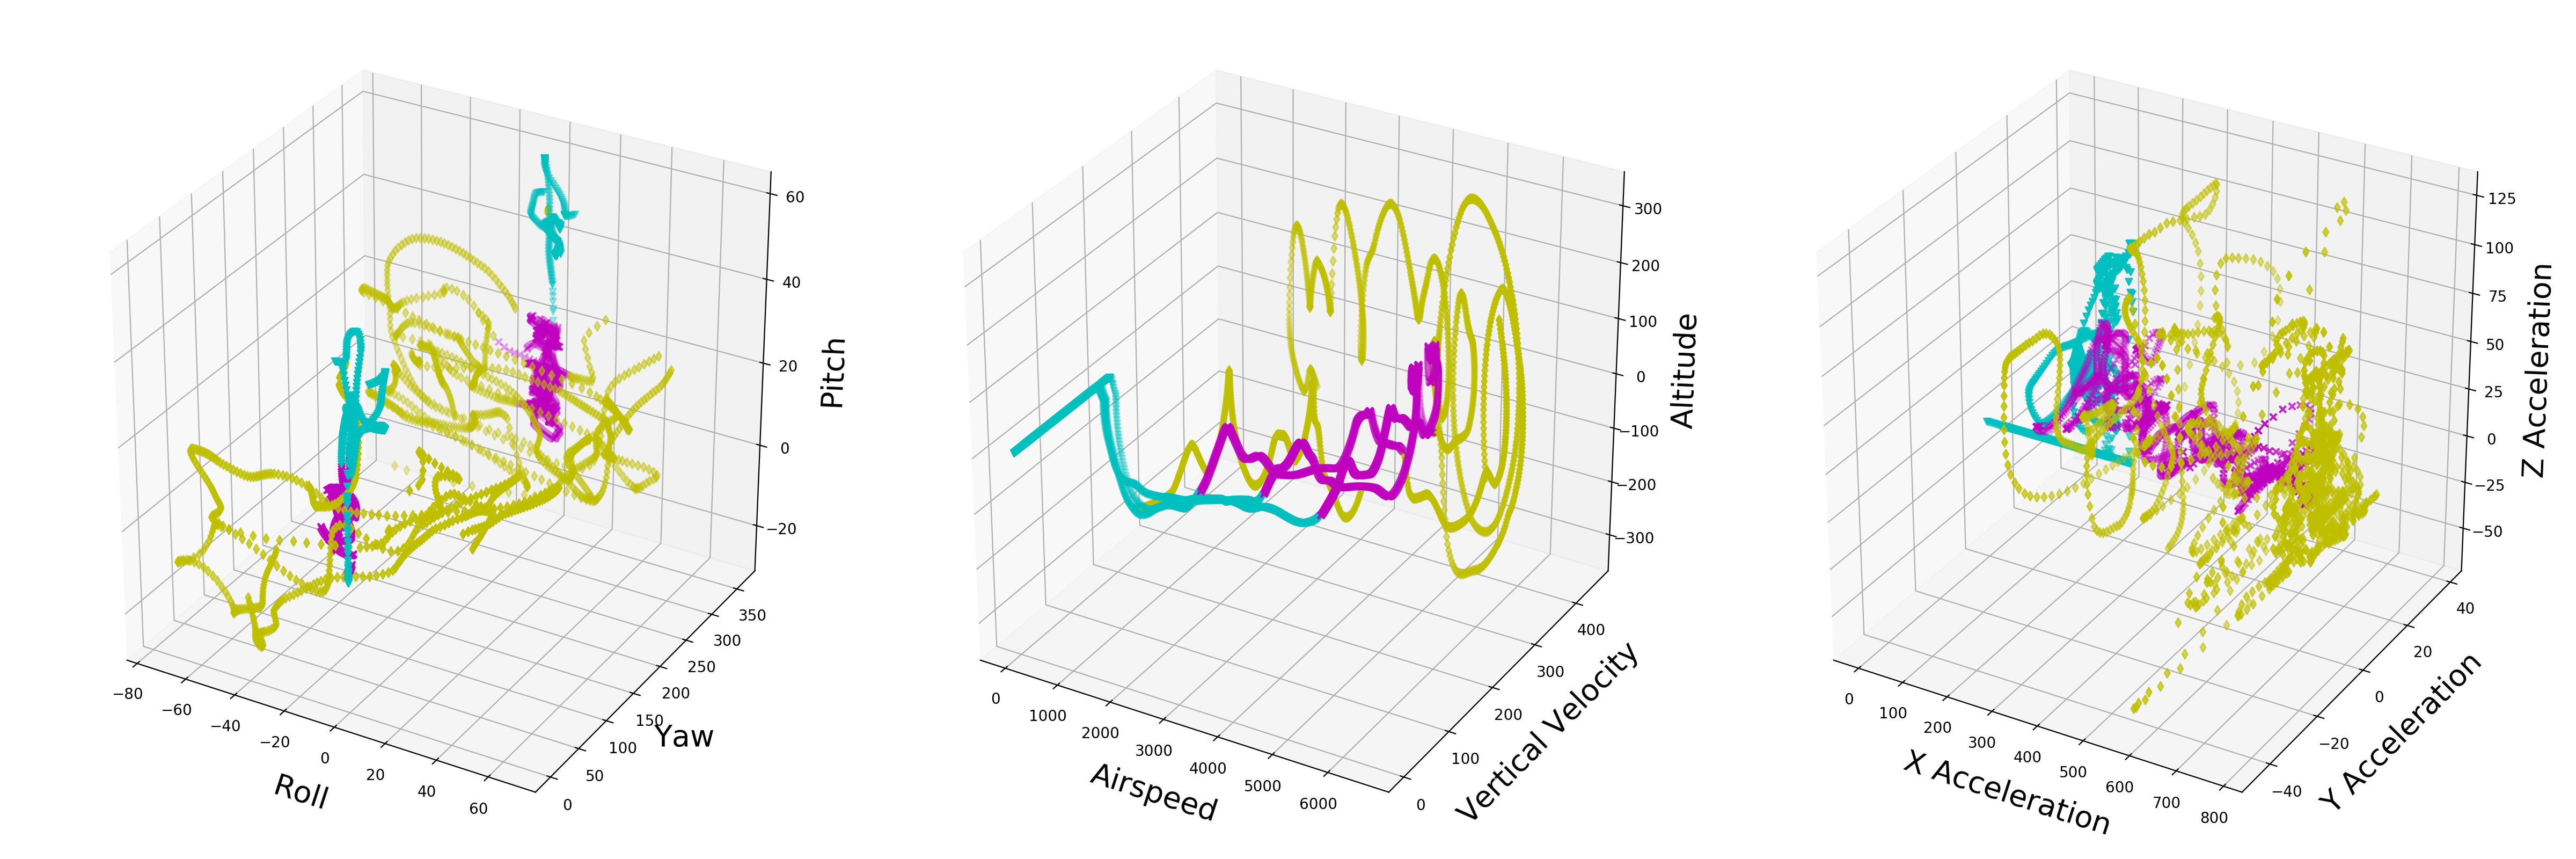
\includegraphics[width=\columnwidth]{3d-plots.png}}
    \caption{Three-dimensional plots for groups of similar features. The takeoff, cruise, and turn classes are shown in cyan, magenta, and yellow, respectively. \textit{Left}: roll vs. yaw vs. pitch. \textit{Middle}: airspeed vs. vertical velocity vs. altitude. \textit{Right}: x-axis acceleration vs. y-axis acceleration vs. z-axis acceleration.}
    \label{fig:3d-plots}
\end{figure}

% hypothesize about important features

Additionally, it is expected that roll, pitch, and yaw are the best predictors of flight maneuvers specifically because the maneuvers in question are essentially \textit{defined} by roll, pitch, and yaw. \figurename \ \ref{fig:3d-plots} supports this hypothesis: clearly, the three classes are most distinct in the left plot. As a secondary objective, then, we examine model performance when all information about the aircraft's orientation is excluded. It is not likely a model which does not use roll, pitch, or yaw data will perform as well as one that does, but we suspect that such a model can still adequately classify flight maneuvers.

\subsection{Model Fitting}

% describe the machine learning task

To compare the model's performance using layman-defined labels to the performance of one that uses expert-defined labels, we need to build the strongest possible classification model. For this reason, multiple classification approaches are evaluated: one-versus-all logistic regression \cite{Bishop2006}, \ac{qda}, the ridge, the random forest classification approach, \ac{knn} classification, and support vector classification \cite{James2013}. In all cases, of course, the fully-labeled dataset means that we conduct fully-supervised learning.

% how are you partitioning the data into train/test sets?

To effectively evaluate the performance of each model, we partition the dataset into training and testing sets using proportional random sampling. Specifically, the training set consists of $90\%$ of the observations from each class; the remaining data points constitute the test set. Because the classes are balanced in the full dataset, they are also balanced in both the training and testing sets.

% cross-validation?

When building the various models, we use $k$-fold \ac{cv}. This ensures that the models are not unnecessarily biased toward the training observations. For $5,000$ observations, $k=10$ is appropriate. This approach certainly increases the model-building complexity (and hence the computation time), but this research requires the best model so that we can effectively evaluate the reliability of human observers; for this reason, we must minimize variance, and thus effective \ac{cv} is necessary. 

% regularization/feature selection?
% iteration to improve results?

\subsection{Feature Selection}

It is certainly possible that some of the available features are not very relevant to maneuver prediction (however, we do not expect this to be the case). Thus, we also conduct feature selection and regularization using best subset selection and the ridge \cite{James2013}. The best subset method is used to fit multiple logistic regression and \ac{qda} models. Various $\alpha$ values are used to fit multiple ridge models. By utilizing both approaches, the likelihood of identifying the best classification model is increased. The extra computational resources required to test two feature selection methods -- instead of just one -- are negligible. In other words, there is not much reason to \textit{not} evaluate both techniques.

\subsection{Iteration}

For each type of classification model, we iterate over the model-fitting parameters until the optimal value is identified. Specifically, we iterate over every possible subset of the set of features for logistic regression and \ac{qda}; over $\alpha$, the strength of the regularization, for ridge classification; over tree depth and $m$, the number of features to consider at each internal node, for the classification forest; over $n$, the number of neighbors to consider, for \ac{knn}; and over the type of kernel and $C$, the classifier's \textit{budget}, for \ac{svc}. (If the \ac{svc} kernel is polynomial, we also iterate over the polynomial degree.)

% I only put this here because I'm lazy; it belongs in 4-Results-Discussion.tex

\begin{figure}
    \centerline{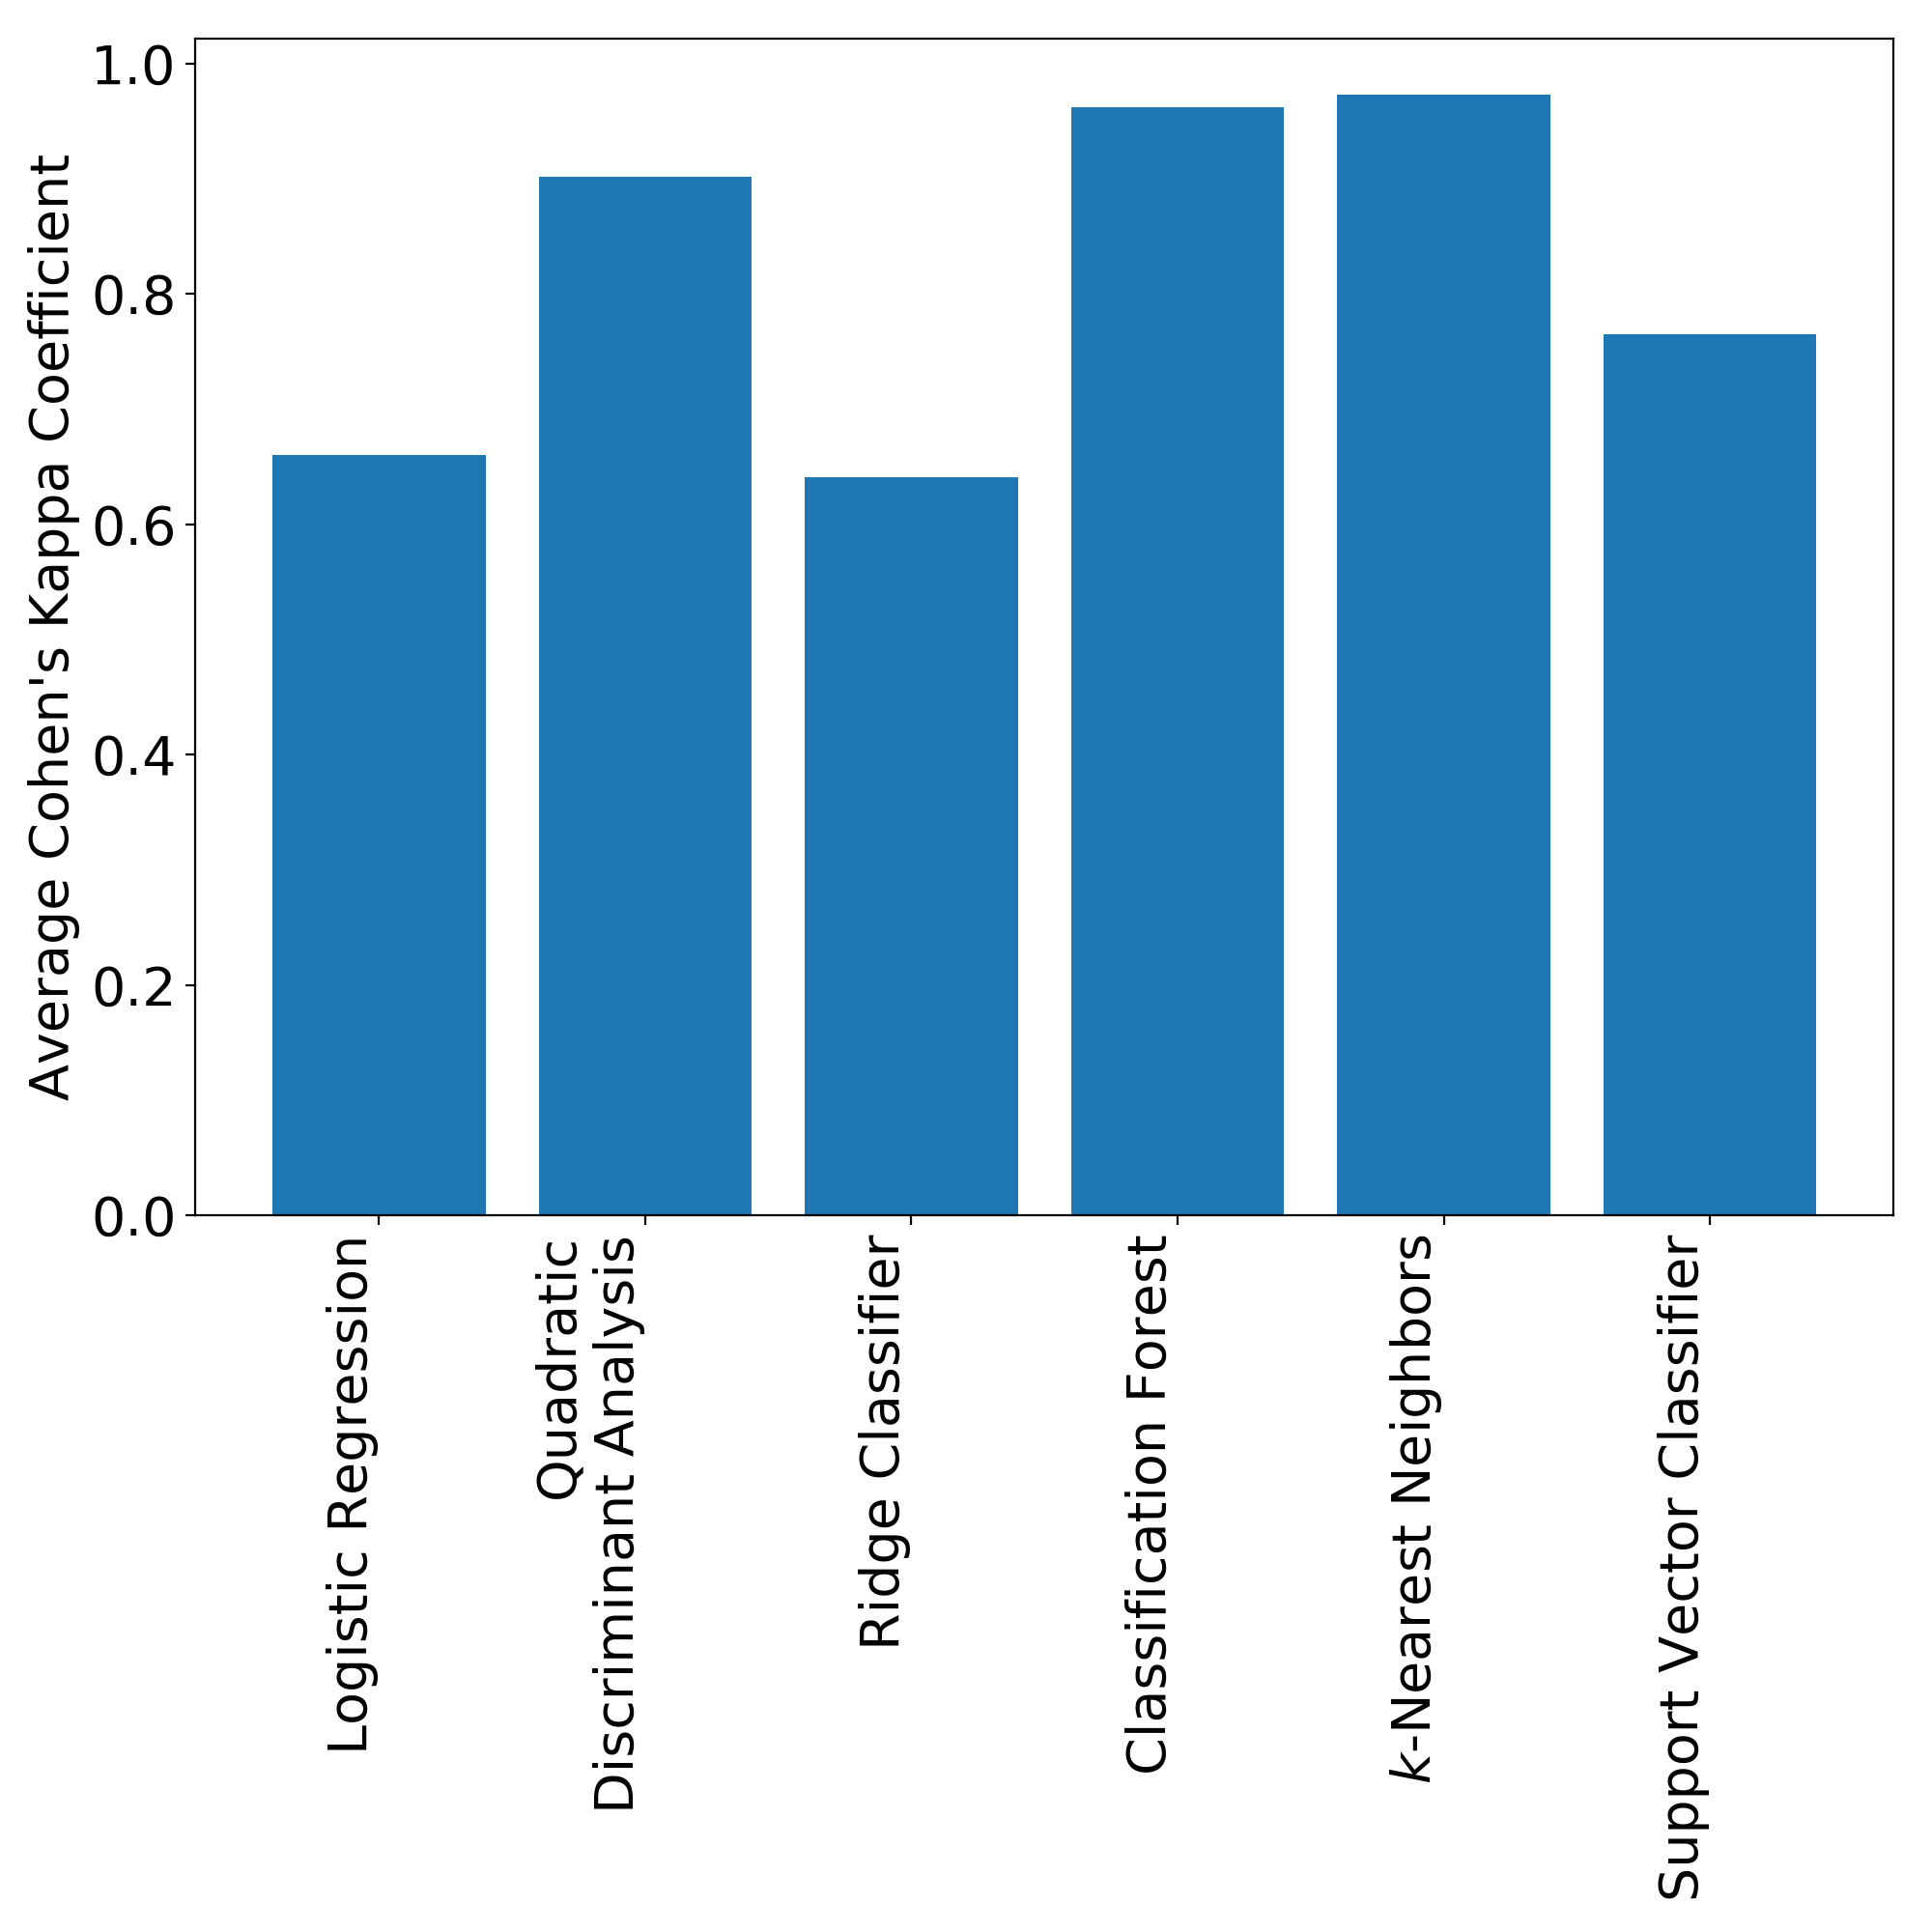
\includegraphics[width=\columnwidth]{ck-bar.png}}
    \caption{Cohen's kappa coefficient averaged over all parameter settings for each of the six types of classifier. These are the $\kappa$ values between models and the layman's labels, as computed on the training set during model fitting.}
    \label{fig:ck-bar}
\end{figure}

\subsection{Model Evaluation \& Analysis}

% comparing models? improving on existing models?

By tuning the models and their parameters, the single best classifier for the dataset is identified. This optimal model is then compared to a simple, expert predictor based solely on roll, pitch, and yaw. Large discrepancies in performance of the two systems indicate that the layman's observations are mislabeled. In other words, large discrepancies imply that non-experts are not reliable in characterizing aircraft maneuvers. Small discrepancies, on the other hand, illustrate that the labels are accurate in most cases.

% evaluation of model or hyperparameter choices?
% confusion matrices? ROC/AUC? accuracy? precision? class imbalances?
% multiple repetition?
% plan for evaluating errors/residuals?

To actually identify the best model and compare it against the expert system, a reliable evaluation procedure is needed. In this research, we utilize Cohen's kappa coefficient \cite{Kappa} to easily compare model performance. For two sets of labels $a$ and $b$, this value is defined by

\[ \kappa = \frac{p_o - p_c}{1 - p_c} = 1 - \frac{1 - p_o}{1 - p_c}, \]

\noindent where $p_o$ is the observed agreement between $a$ and $b$, and $p_c$ is the chance agreement between $a$ and $b$. More details can be found in \cite{Kappa}. We must compute this value for each of the models (that is, each of the model and parameter value combinations), but repeating these computations is trivial. The scores identify the best and worst models, and they also describe the level of agreement between the best model and the expert system.

% transition paragraph

We have now described how the classification performance of each model is evaluated. The following section details the results of the model evaluation. Specifically, it describes which models and parameter settings performed best, and it dicusses what each of various potential results might indicate about the system and about other, less-related systems.

\end{document}